\chapter{Parte 1}
\label{ch:into} % This how you label a chapter and the key (e.g., ch:into) will be used to refer this chapter ``Introduction'' later in the report. 
% the key ``ch:into'' can be used with command \ref{ch:intor} to refere this Chapter.

La soluzione ad attori del problema degli Assignement precedenti è stata implementata in java, utilizzando la libreria Akka.

### Struttura del Sistema ad Attori e Descrizione Operativa

La gerarchia è composta da tre principali livelli di attori: **Boss**, **Pm** e **Employee**, ciascuno con ruoli e responsabilità ben definiti.  

#### Livello 1: Boss  
L'attore **Boss** è la radice della gerarchia ed è responsabile dell'intero processo di gestione dei task. Riceve il percorso di una directory (`directoryPath`) e popola una lista di compiti (`pathList`) utilizzando la funzione `Utils.populateListOfPaths`. Dopo aver suddiviso i compiti in sottogruppi basandosi sul numero di lavoratori disponibili, il **Boss** invia un messaggio `Pm.Order` al suo subordinato **Pm**, specificando:
- La directory di lavoro.
- I compiti da eseguire suddivisi in blocchi.
- Eventuali riferimenti per risposte future.  

Inoltre, il **Boss** monitora l'elaborazione tramite i report inviati dagli **Employee**, aggiornando i dati attraverso un’interfaccia che organizza i risultati dei task. Questo lo rende il punto centrale della raccolta dei risultati.

#### Livello 2: Pm (Project Manager)  
Il **Pm** agisce come intermediario tra il **Boss** e i lavoratori effettivi (**Employee**). Al momento della creazione, genera una serie di attori **Employee**, il cui numero è specificato dalla costante `NUMBER_OF_WORKERS`. Il **Pm** riceve i compiti dal **Boss** e li assegna ai suoi lavoratori utilizzando il messaggio `Ordered`, suddividendo equamente i task.  
Durante l'elaborazione, il **Pm** riceve i report dagli **Employee** tramite messaggi di tipo `Employee.Report` e li inoltra al **Boss**.  
In caso di comandi globali come la pausa (`StopMsg`) o la ripresa (`ResumeMsg`), il **Pm** inoltra i messaggi a tutti gli **Employee**, garantendo un controllo centralizzato.

#### Livello 3: Employee  
Gli attori **Employee** rappresentano i lavoratori del sistema. Ognuno riceve un insieme di compiti dal **Pm** e li elabora uno alla volta. Le principali caratteristiche di un **Employee** includono:
- **Gestione Asincrona dei Task:** I task vengono elaborati utilizzando una funzione di utilità (`Utils.linesWithBufferInputStream`) e i risultati vengono inviati tramite un report al mittente (di norma il **Pm**).
- **Pausa e Ripresa:** Gli **Employee** possono fermare l'elaborazione dei task tramite il messaggio `StopMsg` e riprenderla tramite `ResumeMsg`. Questa capacità migliora la resilienza del sistema e consente una gestione flessibile dei lavoratori.
- **Chiusura Ciclica dei Task:** Utilizzano un iteratore (`taskIterator`) per avanzare nel ciclo di compiti assegnati e inviano notifiche al completamento.

#### Interazione tra gli Attori  
L'interazione tra gli attori è basata su un flusso di messaggi ben definito:
1. **Boss → Pm:** Invio dei compiti tramite `Pm.Order`.
2. **Pm → Employee:** Assegnazione dei task tramite `Ordered`.
3. **Employee → Pm:** Invio dei risultati dei task tramite `Employee.Report`.
4. **Pm → Boss:** Trasmissione dei report degli **Employee**.

Questa struttura modulare rende il sistema scalabile e facile da mantenere, poiché ogni livello si occupa esclusivamente di un insieme ben definito di responsabilità.

#### Vantaggi del Design
1. **Modularità:** Ogni attore ha ruoli chiari, facilitando estensioni o modifiche.
2. **Parallelismo:** L'uso degli attori consente un'elaborazione parallela dei task.
3. **Resilienza:** La gestione di eventi come pause e riprese garantisce continuità operativa.
4. **Scalabilità:** È possibile aggiungere più attori **Pm** o **Employee** per gestire un numero maggiore di compiti senza modificare l'architettura principale.

Se desideri, posso creare una sezione per includere potenziali miglioramenti o una visualizzazione grafica della gerarchia e delle comunicazioni. Fammi sapere!


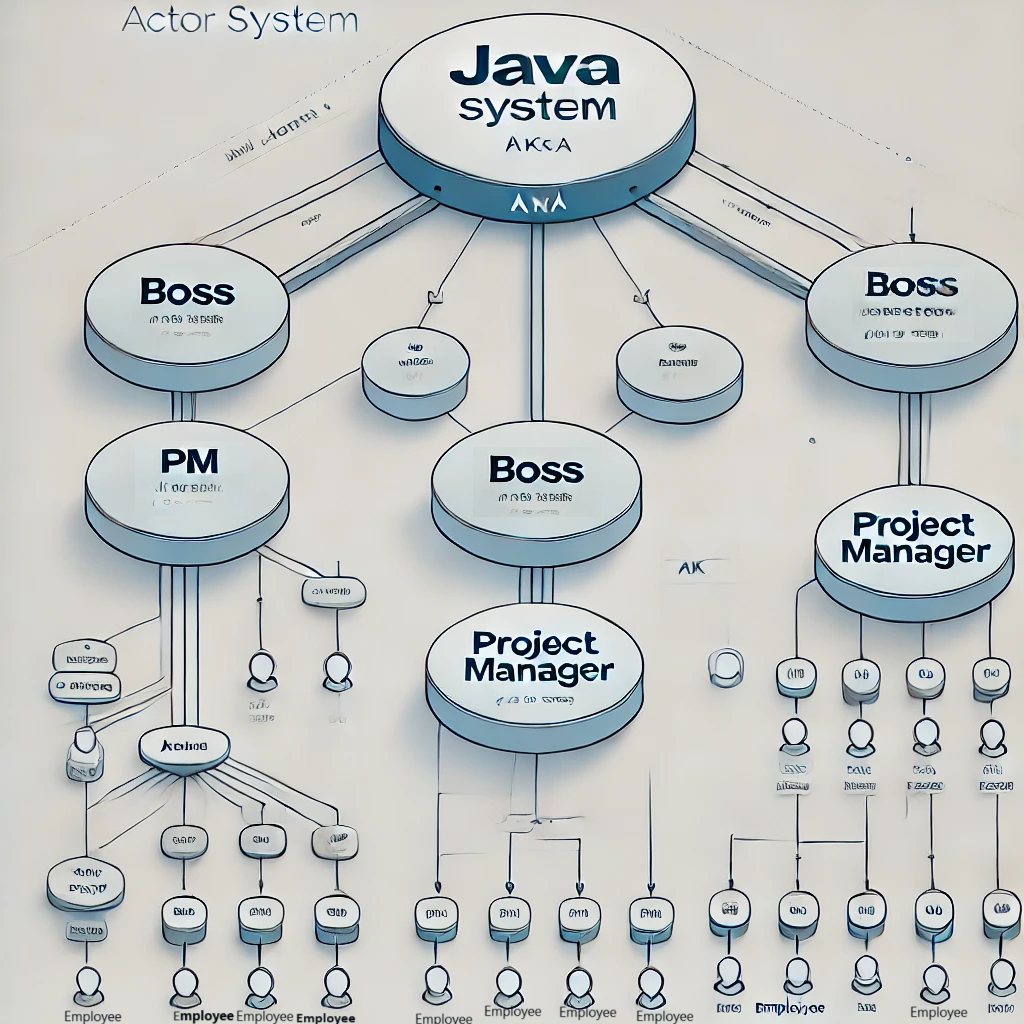
\includegraphics[width=3cm]{/report/imng/chaGpt-graph.png}\\[0.5cm]